\documentclass[journal]{IEEEtran}
\usepackage{cite}
\usepackage{amsmath,amssymb,amsfonts}
\usepackage{graphicx}
\usepackage{algorithm}
\usepackage{algpseudocode}
\usepackage[hidelinks]{hyperref}
\graphicspath{{../../../paper/}}
\makeatletter
\newlabel{sec:system_model}{{II}{1}{}{}{}}
\newlabel{eq:normalized_task_cost}{{30}{1}{}{}{}}
\newlabel{eq:network_service_utility}{{31}{1}{}{}{}}
\newlabel{eq:joint_optimization_problem}{{32}{1}{}{}{}}
\makeatother
\begin{document}
\setcounter{section}{3}
\setcounter{equation}{32}
\setcounter{figure}{1}
\section{Proposed HAN--PDQN Framework}
\label{sec:proposed_framework}

\subsection{Framework Overview}
\label{subsec:framework_overview}

To address \eqref{eq:joint_optimization_problem}, we develop
HAN--PDQN, which connects a representation of multi-user
contention to parameterized satellite and offloading decisions.
As illustrated in Fig.~\ref{fig:han_pdqn_framework}, the
controller constructs a heterogeneous graph from user demand,
satellite resources, and their serving and visibility relations.
HAN aggregates these measurements into a user representation
that distinguishes established resource sharing from potential
competition through overlapping satellite alternatives.

The representation is combined with the user's local task
and candidate-satellite observations. Conditioned on this input,
PDQN generates an offloading fraction for each satellite
action and evaluates the resulting satellite--fraction pairs.
All users share the decision-network parameters, while their
observations and feasible candidates produce different actions.
The joint requests are then executed under the service rules
in Section~\ref{sec:system_model}, yielding task outcomes and
the next network snapshot. Sections~\ref{subsec:han_contention}
and~\ref{subsec:pdqn_joint_control} develop the representation
and decision mechanisms, respectively;
Section~\ref{subsec:training_execution} describes their use
during training and online operation.

\begin{figure*}[t]
    \centering
    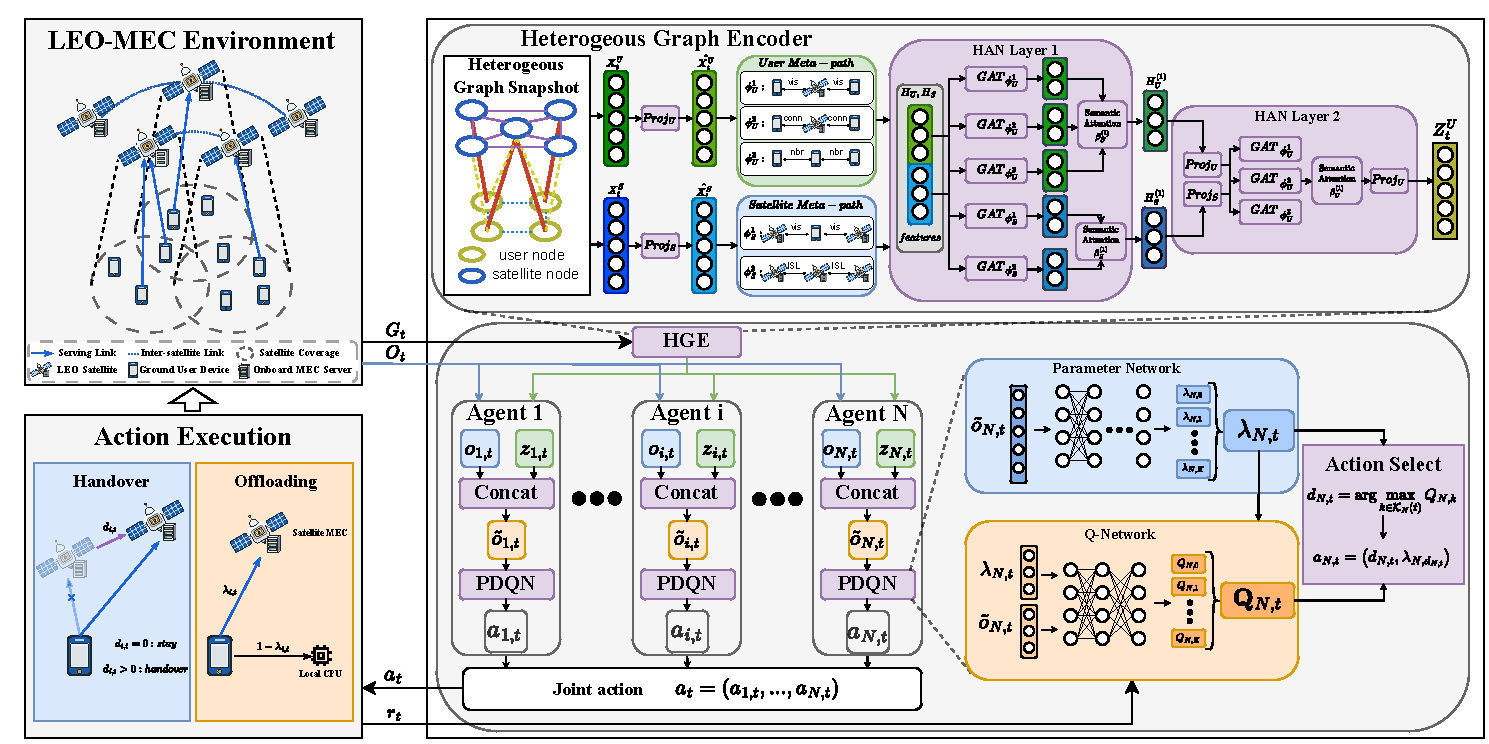
\includegraphics[
        trim=3mm 0.3mm 0.2mm 2mm,
        clip,
        width=\textwidth
    ]{算法框架图10_23.pdf}
    \caption{HAN--PDQN framework for joint handover and partial
    task offloading. The heterogeneous graph encoder produces
    user representations that condition both continuous-parameter
    generation and action-value estimation. The diagram uses
    $\lambda$ for the requested offloading fraction denoted
    by $\widehat{\rho}$ in the text.}
    \label{fig:han_pdqn_framework}
\end{figure*}

\subsection{Heterogeneous Graph-Based Contention Representation}
\label{subsec:han_contention}

At slot $t$, we construct
$\mathcal{G}_t=(\mathcal{V},\mathcal{E}_t,\mathbf{X}_t,
\mathbf{E}_t)$, where $\mathcal{V}$ contains user and satellite
nodes, $\mathcal{E}_t$ contains typed edges, and
$\mathbf{X}_t$ and $\mathbf{E}_t$ collect node and edge
features. User features describe location, connection status,
task demand, urgency, and backlog. Satellite features describe
location, MEC utilization, queue occupancy, associated users,
and available computing resources. Visibility edges carry
distance, elevation, SNR, reference rate, and remaining
visibility; serving edges identify existing associations
and their service duration. Nearby-user and ISL edges provide
geographical and constellation-neighborhood information.
User--satellite relations are represented in both directions.

The five meta-paths in Table~\ref{tab:han_metapaths}
organize these relations into complementary service contexts.
The serving-based U--S--U path aggregates users attached to
the same MEC, exposing established contention. The
visibility-based U--S--U path connects users with common
satellite alternatives, exposing demand that may converge
on the same server after subsequent decisions. This
distinction enables the representation to retain both the
current sharing structure and the opportunities through
which that structure can change. The remaining paths
incorporate neighboring demand, overlapping satellite
coverage, and ISL neighborhoods.

\begin{table}[t]
    \caption{Meta-Paths Used for Contention Representation}
    \label{tab:han_metapaths}
    \centering
    \footnotesize
    \renewcommand{\arraystretch}{1.13}
    \begin{tabular}{p{0.38\columnwidth}p{0.53\columnwidth}}
        \hline
        Meta-path and relation & Service context \\
        \hline
        U--S--U (serving) &
        Users sharing a serving MEC \\
        U--S--U (visibility) &
        Users with common satellite alternatives \\
        U--U (proximity) &
        Demand from neighboring users \\
        S--U--S (visibility) &
        Satellites visible to common users \\
        S--S--S (ISL) &
        Satellite context across two ISL hops \\
        \hline
    \end{tabular}
\end{table}

Following the hierarchical attention principle
in~\cite{wang2019han}, we first aggregate neighbors along
each meta-path and then combine the resulting semantic
representations. At each HAN layer, type-specific projections
map node features into a common hidden space. Each meta-path
starts from these projected features and propagates messages
successively along its constituent relations.

For one relation $r$ at a given meta-path hop, let
$\mathcal{N}_r(v)$ denote the incoming neighbors of node $v$.
For attention head $h$, the score and normalized weight are
\begin{equation}
\begin{aligned}
e_{uv}^{r,h}
&=\operatorname{LeakyReLU}
\left(
(\mathbf{a}^{r,h})^{\mathsf T}
\left[
\mathbf{W}_{\mathrm s}^{r,h}\mathbf{h}_u
\Vert
\mathbf{W}_{\mathrm d}^{r,h}\mathbf{h}_v
\Vert
\mathbf{W}_{\mathrm e}^{r,h}\mathbf{e}_{uv}^{r}
\right]
\right),\\
\alpha_{uv}^{r,h}
&=
\frac{\exp(e_{uv}^{r,h})}
{\sum_{w\in\mathcal{N}_r(v)}
 \exp(e_{wv}^{r,h})},
\end{aligned}
\label{eq:han_relation_attention}
\end{equation}
where $\Vert$ denotes concatenation and
$\mathbf{e}_{uv}^{r}$ is the edge feature.
The matrices and attention vectors are specific to the layer,
meta-path, and hop; these indices are suppressed for clarity.
The $H$ heads produce the message and residual update
\begin{equation}
\begin{aligned}
\mathbf{m}_v^r
&=
\mathop{\Vert}_{h=1}^{H}
\sum_{u\in\mathcal{N}_r(v)}
\alpha_{uv}^{r,h}
\mathbf{W}_{\mathrm s}^{r,h}\mathbf{h}_u,\\
\mathbf{h}_v^{+}
&=
\operatorname{LN}
\left(\mathbf{h}_v+\operatorname{ELU}(\mathbf{m}_v^r)\right).
\end{aligned}
\label{eq:han_hop_update}
\end{equation}
Applying \eqref{eq:han_hop_update} along a meta-path $\phi$
yields its output $\mathbf{h}_v^\phi$.
Thus, user demand is first aggregated at the intermediate
satellite and then propagated to the destination users
on a U--S--U path.

Let $\Phi_\nu$ contain the meta-paths ending at node type
$\nu\in\{\mathrm U,\mathrm S\}$, and let $\mathcal{V}_\nu$
be the corresponding node set. Semantic attention assigns
each applicable path the score
\begin{equation}
w_{\phi,\nu}
=
\frac{1}{|\mathcal{V}_\nu|}
\sum_{v\in\mathcal{V}_\nu}
\mathbf{q}_\nu^{\mathsf T}
\tanh\left(\mathbf{W}_\nu\mathbf{h}_v^\phi
+\mathbf{b}_\nu\right).
\label{eq:han_semantic_score}
\end{equation}
The path weights and fused node representation are
\begin{equation}
\begin{aligned}
\beta_{\phi,\nu}
&=
\frac{\exp(w_{\phi,\nu})}
{\sum_{\phi'\in\Phi_\nu}\exp(w_{\phi',\nu})},\\
\mathbf{z}_v
&=
\mathbf{W}^{\mathrm{out}}_\nu
\sum_{\phi\in\Phi_\nu}
\beta_{\phi,\nu}\mathbf{h}_v^\phi
+\mathbf{b}^{\mathrm{out}}_\nu.
\end{aligned}
\label{eq:han_semantic_fusion}
\end{equation}
These semantic weights are shared by nodes of the same type
within a graph snapshot, while node-level weights depend
on the contributing neighbors.

Stacking HAN layers allows satellite representations formed
through S--U--S and S--S--S paths to enter user-directed
propagation in the next layer. Consequently, the final
user embedding $\mathbf{z}_i(t)$ incorporates the user's
own demand, competing users, and the surrounding satellite
resource context. This embedding supplies the common
relational input to both PDQN components.

\subsection{PDQN-Based Joint Handover and Offloading}
\label{subsec:pdqn_joint_control}

The underlying network state includes orbital conditions,
associations, ordered queues, residual workloads, and local
processor availability. Decisions use the available
measurements summarized in a raw observation
$\mathbf{o}_i(t)$: user and serving-link information,
head-of-line task attributes and urgency, queue backlog,
and the ordered candidate-satellite features.
We combine this observation with the HAN output as
\begin{equation}
\widetilde{\mathbf{o}}_i(t)
=
\left[\mathbf{o}_i(t)\Vert\mathbf{z}_i(t)\right].
\label{eq:fused_pdqn_observation}
\end{equation}
The raw features preserve the task and candidate details,
while $\mathbf{z}_i(t)$ supplies their multi-user context.

The user-level feedback corresponding to
\eqref{eq:network_service_utility} is
\begin{equation}
\begin{aligned}
r_i(t)
={}&
\sum_{n\in\mathcal{Z}_i^{\mathrm{s}}(t)}
(1-c_{i,n})
-|\mathcal{Z}_i^{\mathrm{f}}(t)|\\
&-\omega_{\mathrm I}I_i(t)
-\omega_{\mathrm F}F_i(t)
+\omega_{\mathrm L}J(t).
\end{aligned}
\label{eq:pdqn_user_reward}
\end{equation}
Its arithmetic mean is $U(t)$.
Each user's task and association outcomes therefore provide
local credit, while the load-balance term supplies common
feedback on shared resources.

For a fixed maximum of $K$ candidate slots, let
$s_{i,j}(t)$ be the satellite occupying slot $j$.
The discrete network index is
$d_i(t)\in\{0,\ldots,K\}$, with index $0$ reserved for staying.
It maps to the satellite action in
\eqref{eq:joint_optimization_problem} through
$k_i(t)=0$ for $d_i(t)=0$ and
$k_i(t)=s_{i,d_i(t)}(t)$ otherwise.
Unused candidate slots are masked. The ordered candidate
features, parameter branches, and mask use this same mapping
throughout a decision slot.

Following the parameterized action formulation
in~\cite{xiong2018pdqn}, a branch $\mu_{\psi,j}$ generates
the requested fraction for each discrete index:
\begin{equation}
\widehat{\rho}_{i,j}(t)
=
\mu_{\psi,j}\left(\widetilde{\mathbf{o}}_i(t)\right)
=
\sigma\left(
f_{\psi,j}\left(\widetilde{\mathbf{o}}_i(t)\right)
\right),
\label{eq:pdqn_parameter_generation}
\end{equation}
where $\sigma$ is the sigmoid function and $\psi$ collects
the branch parameters. Branch $0$ controls offloading
through the current association. Requests below the
minimum effective fraction $\rho_{\min}$ invoke local
execution.

The shared Q-network evaluates each complete
index--fraction pair:
\begin{equation}
q_{i,j}(t)
=
Q_\theta\left(
\widetilde{\mathbf{o}}_i(t),j,
\widehat{\rho}_{i,j}(t)
\right).
\label{eq:pdqn_pair_value}
\end{equation}
Its inputs are the fused observation, a one-hot encoding
of $j$, and that branch's scalar fraction.
The output estimates the discounted user return associated
with the requested pair and subsequent decisions.
Both $\psi$ and $\theta$ are shared across users.

Let $m_{i,j}(t)$ indicate whether candidate index $j$
satisfies the current action conditions, and define
$\mathcal{K}_i(t)=\{j:m_{i,j}(t)=1\}$.
The stay index always belongs to $\mathcal{K}_i(t)$.
Online action selection is
\begin{equation}
\begin{aligned}
d_i^\star(t)
&=\arg\max_{j\in\mathcal{K}_i(t)}q_{i,j}(t),\\
\widehat{\rho}_i(t)
&=\widehat{\rho}_{i,d_i^\star(t)}(t).
\end{aligned}
\label{eq:pdqn_joint_selection}
\end{equation}
The sigmoid output satisfies $\mathrm{C}_2$, and the mask
implements the candidate, trigger, link, and migration
checks in $\mathrm{C}_1$ and $\mathrm{C}_3$--$\mathrm{C}_5$.
The execution-stage admission rules enforce
$\mathrm{C}_6$ as users share the remaining capacity.

Equations~\eqref{eq:pdqn_parameter_generation}
and~\eqref{eq:pdqn_pair_value} expose the coupling between
representation and control: the same contention information
conditions both the workload proposed for a candidate and
the estimated value of assigning that workload to it.
The final selection therefore compares satellite actions
together with their associated continuous fractions.

\subsection{Training and Online Execution}
\label{subsec:training_execution}

Training uses an experience replay buffer $\mathcal{D}$
of joint transitions, each containing the user tuples
$(\widetilde{\mathbf{o}},d,\widehat{\rho},r,
\widetilde{\mathbf{o}}',\delta,\mathbf{m},\mathbf{m}')$.
Here, $\widehat{\rho}$ is the requested fraction,
the primed quantities describe the next observation,
and $\delta$ indicates a true terminal transition.
The buffer stores the encoded observations used for
the decisions. A minibatch of $B$ joint transitions
provides $BN$ user samples for the shared PDQN networks.

Task feedback is assigned when an outcome is resolved.
For local-only execution, the reserved completion time
determines the outcome at dispatch; remote outcomes
are evaluated upon MEC completion, expiration, or
termination. Interruption, association-failure, and
load-balance feedback are assigned in the corresponding
slot. Thus, the replay reward follows
\eqref{eq:pdqn_user_reward}, including outcomes from
previously dispatched workloads.

Let $Q_{\bar{\theta}}$ and $\mu_{\bar{\psi},j}$
denote the target networks. For a sampled next observation,
the online networks select
\begin{equation}
d'
=
\arg\max_{j:m'_j=1}
Q_\theta\left(
\widetilde{\mathbf{o}}',j,
\mu_{\psi,j}(\widetilde{\mathbf{o}}')
\right).
\label{eq:pdqn_next_action}
\end{equation}
The target networks then evaluate this choice:
\begin{equation}
y
=
r+\gamma(1-\delta)
Q_{\bar{\theta}}\left(
\widetilde{\mathbf{o}}',d',
\mu_{\bar{\psi},d'}(\widetilde{\mathbf{o}}')
\right).
\label{eq:pdqn_td_target}
\end{equation}
The Q-network minimizes
\begin{equation}
\mathcal{L}_Q(\theta)
=
\mathbb{E}_{\mathcal{D}}
\left[
\left(
Q_\theta(\widetilde{\mathbf{o}},d,\widehat{\rho})-y
\right)^2
\right].
\label{eq:pdqn_q_loss}
\end{equation}
Time-limit truncation retains bootstrapping, since
unfinished workloads continue to have future value.

The parameter branches are updated through the Q-network
using the objective
\begin{equation}
\mathcal{L}_{\mu}(\psi)
=
-\eta_{\mu}
\mathbb{E}_{\mathcal{D}}
\left[
\max_{j:m_j=1}
Q_\theta\left(
\widetilde{\mathbf{o}},j,
\mu_{\psi,j}(\widetilde{\mathbf{o}})
\right)
\right],
\label{eq:pdqn_parameter_loss}
\end{equation}
where $\eta_{\mu}>0$ scales the parameter objective.
During this update, $\theta$ is held constant and
gradients propagate through the continuous parameter
of the maximizing feasible branch.
Both optimizers use gradient clipping.
Every $C_{\mathrm{tar}}$ learning updates, the target
parameters are copied from the online networks:
$\bar{\theta}\leftarrow\theta$ and
$\bar{\psi}\leftarrow\psi$.

Exploration samples a feasible discrete index and a
continuous fraction uniformly from $[0,1]$.
After the initial replay warm-up, this random pair is
selected with probability $\epsilon$; otherwise, the
controller uses \eqref{eq:pdqn_joint_selection}.
The exploration probability decreases during training.
Algorithm~\ref{alg:han_pdqn_training} summarizes the procedure.

\begin{algorithm}[t]
\caption{HAN--PDQN Training}
\label{alg:han_pdqn_training}
\begin{algorithmic}[1]
\Require HAN encoder, candidate limit $K$, replay capacity,
batch size $B$, target period $C_{\mathrm{tar}}$
\State Initialize $\theta,\psi$ and replay buffer $\mathcal{D}$
\State Set $\bar{\theta}\gets\theta$, $\bar{\psi}\gets\psi$
\For{each training episode}
    \State Reset the environment and construct $\mathcal{G}_0$
    \State Form $\widetilde{\mathbf{o}}_i(0)$ and
    $\mathbf{m}_i(0)$ for all users
    \For{each decision slot $t$}
        \For{each user $i\in\mathcal{U}$}
            \State Select a feasible pair by exploration or
            \eqref{eq:pdqn_joint_selection}
        \EndFor
        \State Execute the joint requests under the service model
        \State Obtain $r_i(t)$, $\widetilde{\mathbf{o}}_i(t+1)$,
        and $\mathbf{m}_i(t+1)$
        \State Store the joint transition in $\mathcal{D}$
        \If{replay warm-up is complete}
            \State Sample a minibatch from $\mathcal{D}$
            \State Compute targets using
            \eqref{eq:pdqn_next_action}--\eqref{eq:pdqn_td_target}
            \State Update $\theta$ using \eqref{eq:pdqn_q_loss}
            \State Update $\psi$ using \eqref{eq:pdqn_parameter_loss}
            \State Copy online parameters to targets every
            $C_{\mathrm{tar}}$ updates
        \EndIf
        \If{episode terminates or reaches its time limit}
            \State \textbf{break}
        \EndIf
    \EndFor
\EndFor
\end{algorithmic}
\end{algorithm}

For online operation, the controller constructs the graph,
computes the fused user observations, and selects the
masked maximizing pairs with $\epsilon=0$.
Association changes are resolved before new upload
requests are admitted and allocated bandwidth, following
Section~\ref{sec:system_model}.
This sequence preserves the candidate mapping used
at decision time while applying capacity checks to
the committed actions.

For computational cost, let $L$ be the number of HAN
layers and $D_{\mathrm h}$ the hidden width.
Let $V_{\mathrm{mp}}$ and $E_{\mathrm{mp}}$ count node
and edge visits across the meta-path hops in one layer.
For a fixed number of heads, graph encoding requires
$O(L(V_{\mathrm{mp}}D_{\mathrm h}^2+
E_{\mathrm{mp}}D_{\mathrm h}))$ operations.
If $P_\mu$ is the total parameter-branch weight count
and $P_Q$ is the Q-network weight count, evaluating all
users adds $O(N[P_\mu+(K+1)P_Q])$.
A replay update over $B$ joint transitions has network cost
$O(BN[P_\mu+(K+1)P_Q])$.
Graph construction contributes a separate cost determined
by visibility and neighborhood generation.
Online execution uses graph construction, encoding,
and forward action evaluation; replay updates contribute
to training cost.

\begin{thebibliography}{2}
\bibitem{wang2019han} X. Wang et al., Heterogeneous Graph Attention Network, 2019.
\bibitem{xiong2018pdqn} J. Xiong et al., Parameterized Deep Q-Networks for Reinforcement Learning with Hybrid Action Space, 2018.
\end{thebibliography}
\end{document}
